% !TeX root = ../01_Projektarbeit/01_main.tex
\chapter{How To / Anleitung}

Für einen Abschnitt nutzt man \verb|\abschnitt| (selbstdeklarierter Befehl in 01\_main.tex)

\abschnitt{Anleitung}

Zum \textit{kursiv} schreiben nutzt man \verb|\textit{}|
\newline

Um Akronyme einzufügen, müssen diese vorher selbstständig in 01\_main.tex deklariert werden.
\newline

Zitierstil für Kommentare muss noch geändert werden da in der Fußnote folgendes erscheint: "NACHNAME, 2026," > nach dem Jahr steht ein unnötiges Komma.
\newline

Um eine neue Zeile zu beginnen, muss man im Quellcode eine LEERZEILE lassen.
\newline

\verb|\newline| für eine Textumbruch ohne Formatierung der Zeile.
\newline

\verb|\linebreak| für einen Textumbruch bei dem die Zeilenfüllung formatiert wird bzw. richtet den Text als Blocksatz aus
\newline

für eine leerzeile schreibt man \verb|\\| am ende der zeile und drückt dann 2x Return
\verb|\enquote| für Zitate wie z.\,B. \enquote{Hallo}, man kann auch \verb|\enquote| in einem \verb|enquote| benutzen: \enquote{Hier ist noch ein \enquote{enquote} drin}
\newline

für z.\,B. nutzt man \verb|z.\,B| also: z.\,B
\newline

mit einem \verb|\label{eigene bezeichnung:eigener labelname}| kann man einen verlinkung setzen z.\,B. hier mit label abschnitt:unterkapitel, für die Referenz nutzt man \linebreak \verb|~\ref{abschnitt:unterkapitel}|. z.\,B. so hier: Siehe Kapitel ~\ref{abschnitt:unterkapitel}
\newline

Wenn man Einträge in literatur.bib ändert oder eine neue Fußnote schreibt muss man immer ein mal biber laufen lassen
\newline

Arten von Fußnoten / Auflistung mit Zahlen:
\begin{enumerate}[nosep]
	\item \verb|\footvgl[Seite der Quelle]{Name der Quelle in literatur.bib}|: für indirekte Zitate\footvgl[34]{Buch1}
	\item \verb|\footdirekt[Seite der Quelle]{Name der Quelle in literatur.bib}|: für direkte Zitate\footdirekt[3]{Buch3}
	\item \verb|\footonline{Name der Online-Quelle in literatur.bib}|: für Zitate aus Online-Quellen\footonline{OnlineQuelle1}
	\item \verb|\footunpub{Name des Dokuments/Quelle in literatur.bib| für unveröffentlichte Dokumente\footunpub{intern}
\end{enumerate}
Die Fußnoten sind selbstständig definierte Befehle, zu finden in 01\_main.tex.
\newline

Auflistung mit Stichpunkten:
\begin{itemize}[nosep, label=-]
	\item erster Stichpunkt
	\item zweiter Stichpunkt
	\item mit Label stellt man das Stichpunktzeichen ein\newline
\end{itemize}

Abstände im Abbildungsverzeichnis sind größer wenn sich die Abbildungen in unterschiedlichen Kapiteln befinden.
\newline

Wenn ein Akronym \enquote{Underfoll box} verursacht kann man das nehmen:

\verb|\setlength{\emergencystretch}{1em}% ACRO sorgt für underfull box|


\clearpage

\section{Unterkapitel Beispiel}
\label{abschnitt:unterkapitel}
Beispieltext mit Beispielakronym: \ac{Beispielacro}.Referenz zu dem Bild einer kleinen Mieze: Abbildung~\ref{fig:Kitten Eins}. Dieser Satz endet mit einer Fußnote\footvgl[24]{Buch1}.
\begin{figure}[htbp]
	\centering
	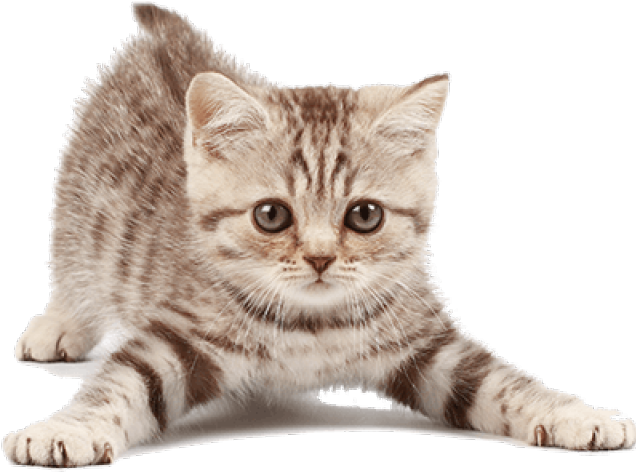
\includegraphics[width=0.5\textwidth]{../03_Bilder/kitten_1.jpg}
	\caption[Süßes Kätzchen 1]{Süßes Kätzchen 1

	{\fontsize{10}{12}\selectfont (Eigene Darstellung)}}
	\label{fig:Kitten Eins}
\end{figure}

Tabelle~\ref{tab:Beispieldaten} zeigt eine Beispieltabelle:
\begin{table}[htbp]
	\centering
	\renewcommand{\arraystretch}{1.3}
		\begin{tabular}{l|l}
			\textbf{Beispielspalte 1} & \textbf{Beispielspalte 2} \\
			\hline
			Spaltentrennung wird mit \verb|&| gemacht -> &
			um in die nächste Zeile zu gehen nutzt man \verb|\\| \\
			\hline
			So kann man hier &
			schöne Sachen hereinschreiben \\
			als Label wurde hier &
			\verb|label{tab:...}| verwendet
		\end{tabular}
		\caption[Beispieldaten]{%
			Beispieldaten\\
			{\fontsize{10}{12}\selectfont (Fiktiv)}%
		}
		\label{tab:Beispieldaten}
\end{table}
\clearpage
